\documentclass{beamer}
\usepackage{pgfplots}
\usetheme{Boadilla}
 
 
\title{Analizador Lexico}
\subtitle{Proyecto 1}
\author{Ariana Bermudez,Ximena Bolanos, Dylan Rodriguez}
\institute{Instituto Tecnologico de Costa Rica}
\date{\today}
\begin{document}
\begin{frame}
\textcolor{yellow}{/*hola*/} \textcolor{blue}{int} \textcolor{green}{i} \textcolor{pink}{=} \textcolor{red}{0} \textcolor{purple}{;} \textcolor{blue}{while} \textcolor{purple}{(} \textcolor{green}{i} \textcolor{pink}{<} \textcolor{red}{10} \textcolor{purple}{)} \textcolor{purple}{{} \textcolor{green}{i} \textcolor{pink}{++} \textcolor{purple}{;} \textcolor{purple}{}} \textcolor{white}{} \end{frame}
\begin{frame}
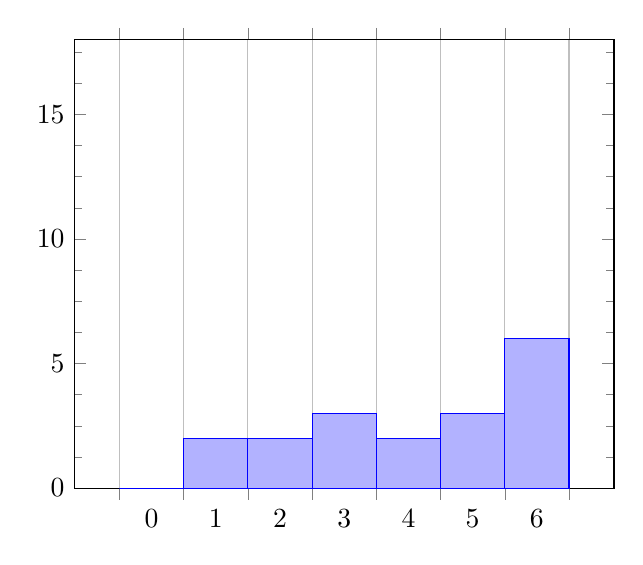
\begin{tikzpicture}
\begin{axis}[ybar interval, ymax=18, ymin=0, minor y tick num = 3]
\addplot coordinates { (0 , 0) (1 , 2) (2 , 2) (3 , 3) (4 , 2) (5 , 3) (6 , 6)  (7, 0) }; 
\end{axis}
\end{tikzpicture}
\end{frame}
\begin{frame}
\def\angle{0}
\def\radius{3}
\def\cyclelist{{"yellow","blue","red","green"}}
\newcount\cyclecount \cyclecount=-1
\newcount\ind \ind=-1
\begin{tikzpicture}[nodes = {font=\sffamily}]
\foreach \percent/\name in {
0/NULL,
11/KEYWORD,
11/INTEGER,
16/IDENTIFIER,
11/CONSTANT,
16/OPERATOR,
33/PUNTUACTOR
 } {
\ifx\percent\empty\else
\global\advance\cyclecount by 1
\global\advance\ind by 1
\ifnum3<\cyclecount
\global\cyclecount=0
\global\ind=0
\fi
\pgfmathparse{\cyclelist[\the\ind]}
\edef\color{\pgfmathresult}
\draw[fill={\color!50},draw={\color}] (0,0) -- (\angle:\radius)
arc (\angle:\angle+\percent*3.6:\radius) -- cycle;
\node at (\angle+0.5*\percent*3.6:0.7*\radius) {\percent\,\%};
\node[pin=\angle+0.5*\percent*3.6:\name]
at (\angle+0.5*\percent*3.6:\radius) {};
\pgfmathparse{\angle+\percent*3.6}
\xdef\angle{\pgfmathresult} % and store in \angle
\fi
};
\end{tikzpicture}

\end{frame}
\end{document}
